\item O pêndulo da máquina de impacto Charpy tem massa de 50 kg e um raio de giração $k_{A}=\SI{1.75}{\meter}$. Se ele é
solto do repouso quando $\theta=0^{\circ}$, determine sua velocidade angular logo antes de atingir o corpo de prova
$S$, $\theta=90^{\circ}$.

\import{../answers}{answer-3}

\vspace{-1cm}
\begin{flushright}
	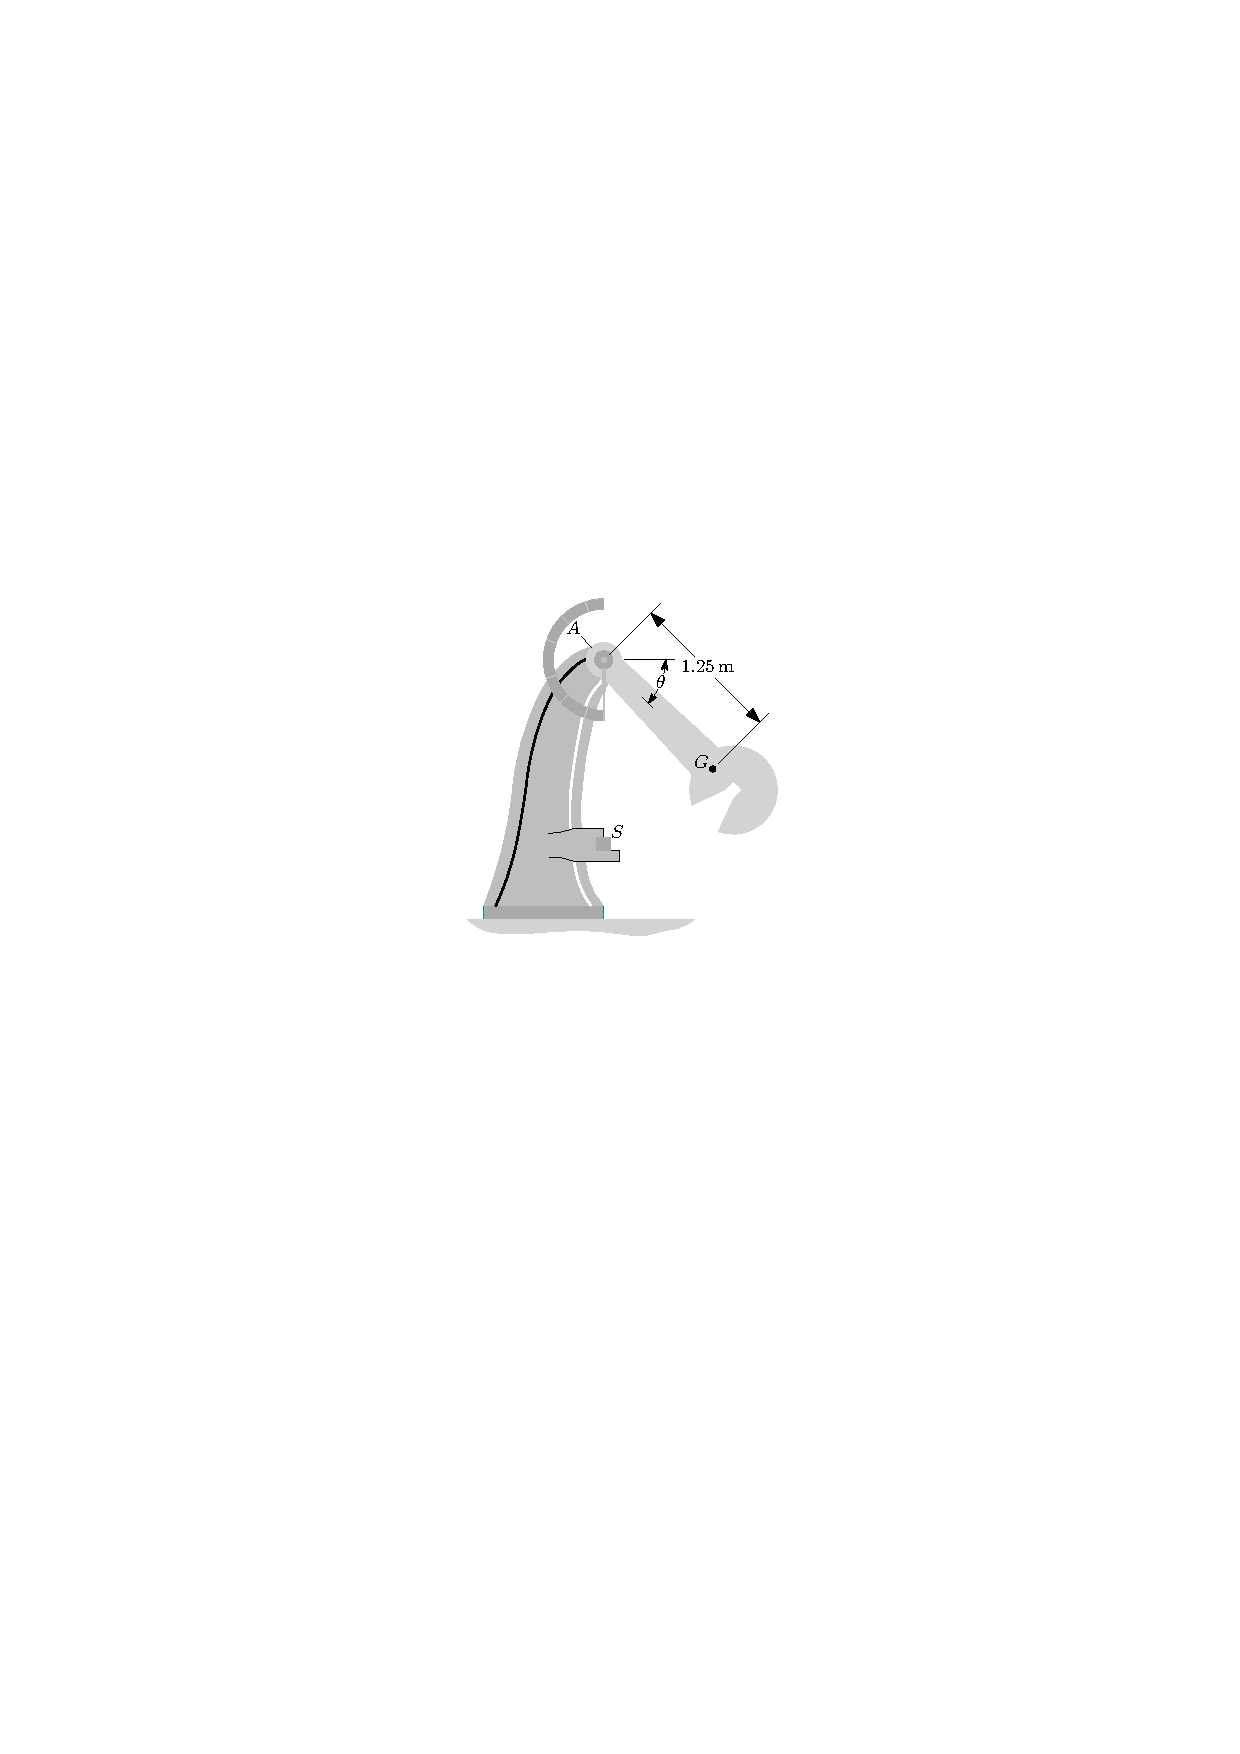
\includegraphics[scale=1.3]{../../images/draw_2}
\end{flushright}